\documentclass[12pt, oneside, a4paper]{report}
\usepackage{graphicx}
\graphicspath{{images/}}

\title{PAGE REPLACEMENT IN VMSIM}
\author{Ananya R \and Chirag Jamadagni}

\begin{document}
\maketitle
\tableofcontents
\newpage

\section*{INTRODUCTION}
\addcontentsline{toc}{section}{INTRODUCTION}
\textbf{What is memory management?}
\\*
Memory management is the functionality of an operating system which handles or manages primary memory. Memory management keeps track of each and every memory location, either it is allocated to some process or it is free. It checks how much memory is to be allocated to each process. It decides which process will get how much memory and at what time[5]. It tracks whenever some memory gets freed or unallocated and correspondingly updates its status.

\subsection*{VIRTUAL MEMORY}
\addcontentsline{toc}{subsection}{VIRTUAL MEMORY}
In computing, virtual memory is a memory management technique that is implemented using both hardware and software. It maps memory addresses used by a program, called virtual addresses, into physical addresses in computer memory. Main storage as seen by a process or task appears as a contiguous address space or collection of contiguous segments. The operating system manages virtual address spaces and the assignment of real memory to virtual memory. Address translation hardware in the CPU, often referred to as a memory management unit or MMU, automatically translates virtual addresses to physical addresses. Software within the operating system may extend these capabilities to provide a virtual address space that can exceed the capacity of real memory and thus reference more memory than is physically present in the computer[6].
\\*
\\*
\textbf{Advantages of implementing Virtual Memory}
\begin{itemize}
\item Freeing applications from having to manage a shared memory space
\item Increased security due to memory isolation
\item Being able to conceptually use more memory than might be physically available, using the technique of paging
\end{itemize}
\newpage

\section*{PAGING AND PAGE REPLACEMENT}
\addcontentsline{toc}{section}{PAGING AND PAGE REPLACEMENT}
\subsection*{PAGING}
\addcontentsline{toc}{subsection}{PAGING}
In computer operating systems, paging is one of the memory management schemes by which a computer stores and retrieves data from the secondary storage for use in main memory. In the paging memory-management scheme, the operating system retrieves data from secondary storage in same-size blocks called pages. The main advantage of paging over memory segmentation is that it allows the physical address space of a process to be non-contiguous. Before paging came into use, systems had to fit whole programs into storage contiguously, which caused various storage and fragmentation problems[3].
\\*
\\*
Paging is an important part of virtual memory implementation in most contemporary general-purpose operating systems, allowing them to use secondary storage for data that does not fit into physical random-access memory (RAM).

\subsection*{PAGE REPLACEMENT}
\addcontentsline{toc}{subsection}{PAGE REPLACEMENT}
\textbf{Page Replacement Algorithms}
\\*
Page replacement algorithms are the techniques using which Operating System decides which memory pages to swap out, write to disk when a page of memory needs to be allocated. Paging happens whenever a page fault occurs and a free page cannot be used for allocation purpose accounting to reason that pages are not available or the number of free pages is lower than required pages.
\\*
\\*
When the page that was selected for replacement and was paged out, is referenced again then it has to read in from disk, and this requires for I/O completion. This process determines the quality of the page replacement algorithm: the lesser the time waiting for page-ins, the better is the algorithm. A page replacement algorithm looks at the limited information about accessing the pages provided by hardware, and tries to select which pages should be replaced to minimize the total number of page misses, while balancing it with the costs of primary storage and processor time of the algorithm itself. There are many different page replacement algorithms. We evaluate an algorithm by running it on a particular string of memory reference and computing the number of page faults.
\\*
\\*
\textbf{The (h,k) paging problem}
\\*
The (h,k)-paging problem is a generalization of the model of paging problem: Let h and k be positive integers such that h<=k. We measure the performance of an algorithm with cache of size h<=k relative to the theoretically optimal page replacement algorithm. If h<k we provide the optimal page replacement algorithm with strictly less resource.
\\*
The (h,k)-paging problem is a way to measure how an online algorithm performs by comparing it with the performance of the optimal algorithm, specifically, separately parameterizing the cache size of the online algorithm and optimal algorithm[4].
\newpage

\section*{VMSIM}
\addcontentsline{toc}{section}{VMSIM}
\textbf{Vmsim} is a virtual memory simulator. It works/runs as a user level process in Linux based operating systems. The installation procedure has been mentioned later. There are many versions of vmsim. Vmsim isn't patented by any organization and therefore there are many versions/implementations of this tool. Each version is independent of the other. For this project we use a version of vmsim written in C language and developed by researchers at the University of Washington[1].

\subsection*{AIM OF THE PROJECT}
\addcontentsline{toc}{subsection}{AIM OF THE PROJECT}
To understand the given skeleton code and create a fault handler which will implement multiple page replacement algorithms. Number of memory frames, input file and the algorithm to be used should be provided by the user.  Appropriate code should be added in all files to successfully simulate page replacement.
\\*
\\*
A very basic and incomplete skeleton implementation of the following components:
\begin{itemize}
\item Physical memory
\item Page table
\item The main simulator
\end{itemize}

\subsection*{INSTALLATION}
\addcontentsline{toc}{subsection}{INSTALLATION}
The Vmsim skeleton can be installed on any Linux distribution by following the below mentioned steps[2].
\\*
\\*
\$ wget http://www.cs.sfu.ca/CourseCentral/300/zonghuag/projects/vmsim.tar.gz
\\*
\$ tar -xxvf vmsim.tar.gz
\\*
\$ cd vmsim
\\*
\$ make
\\*
\$ ./vmsim -h (will tell you how to run the simulator and the arguments/options it takes)

\subsection*{IMPLEMENTATION}
\addcontentsline{toc}{subsection}{IMPLEMENTATION}
\begin{itemize}

\item \textbf{vmsim.c} is responsible for the complete simulation. It contains some initialization code and the simulate() function. This functions reads one memory reference at a time from the input trace file, searches for it in the page table, invokes a page fault handler if not found, and updates some statistics.

\item \textbf{fault.c} contains the page fault handlers.

\item \textbf{stats.c} contains functions to collect and print simulation statistics.

\item \textbf{pagetable.c} contains the implementation of a page table with multiple levels.

\item \textbf{physmem.c} is the structure to represent physical memory along with some functions, i.e load() and evict(). evict() is used to remove a particular page from physical memory. load() is used to load a given page into the physical memory slot. This slot should be empty.

\item \textbf{options.c} contains functions to process command line arguments.

\item \textbf{util.c} contains some additional utility functions.
\\*
\end{itemize}
\\*
\underline{\textbf{Modes of Execution}}
\begin{enumerate}
\item \textbf{Debug Mode}
\\*
\\*
The file options.h has a debug flag. If that flag is enabled the system will execute in debug mode. This mode is mainly used for debugging purposes. After every fault/hit the contents of main memory and the list of all pages which have been loaded into the page table is displayed.
\item \textbf{Normal Mode}
\\*
\\*
If the debug flag is disabled the system executes in this mode. This mode is mainly used for comparison purposes. The simulation statistics are displayed. These include the number of memory references, faults and dirty page writes.
\\*
\end{enumerate}   
\\*
\underline{\textbf{Simulation procedure}}
\\*
\\*
In vmsim.c, the main function simulates the working of a virtual memory unit: It reads memory references (from a trace file) and checks whether this reference is in memory. If it is in the memory, some statistics are updated. If it is not in memory, a page fault occurs and the page fault handler is invoked. The page fault handler uses the replacement policy to evict a page from the memory to make room for the requested page. Several replacement policies can be used with the simulator. The replacement policy should be specified when the simulator is executed. (Refer output of ./vmsim -h)
\\*
\\*
\underline{\textbf{Input file format}}
\\*
\\*
The input file contains the trace data. An example of this data would be 1, R, 0x0000E00. The data is in the format [Process ID], [Mode], [Virtual Address]. The mode can be set to 'R' or 'W' which stand for read and write respectively. We accept the process ID to distinguish between the page tables of different processes. 'Mode' is mainly used for collecting statistics.
\\*
\\*
\underline{\textbf{Components Associated with every Page table entry}}
\\*
\begin{itemize}
\item \textbf{Vfn:} Stands for virtual frame number. This frame is mapped to the virtual memory
\item \textbf{Pfn:} Stands for physical frame number. This frame is mapped to the physical memory (registers).
\item \textbf{Valid:} This is of type Boolean. Set to true if the entry is present in one of the physical memory frames.
\item \textbf{Counter:} An integer variable used to determine the least recently used page for the LRU replacement algorithm.
\item \textbf{Frequency:} Determines the number of hits on an entry present in main memory.
\item \textbf{Used:} Used to represent the used bit for the clock replacement algorithm.
\item \textbf{Chance:} Represents the modification bit for the second chance replacement algorithm.
\item \textbf{Reference Counter (c):} Used to maintain FIFO order for the LFU, MFU and FIFO page replacement algorithms. Represents the position/number at which an entry is added to the table.
\end{itemize}
\newpage

\section*{IMPLEMENTED PAGE REPLACEMENT ALGORITHMS}
\addcontentsline{toc}{section}{IMPLEMENTED PAGE REPLACEMENT ALGORITHMS}
\begin{enumerate}
\item \textbf{First In First Out (FIFO)}
\item \textbf{Least Recently Used (LRU)}
\item \textbf{Least Frequently Used (LFU)}
\item \textbf{Most Frequently Used (MFU)}
\item \textbf{Clock}
\item \textbf{Second Chance}
\item \textbf{Random}
\end{enumerate}

\subsection*{EXECUTION PROCEDURE}
\addcontentsline{toc}{subsection}{EXECUTION PROCEDURE}
\begin{enumerate}
\item Change the present working directory to the “vmsim” folder.
\\*
\item To compile the code type the command “make” or “gmake” in the terminal window.
\\*
\item To view which page replacement algorithms can be used and other options type “./vmsim -h”
\\*
\item The following statement is an example for testing the virtual memory simulation where the input is read from the exampletrace.txt file.
\\*
./vmsim -p 3 -s 32 random exampletrace.txt
\\*
Where, '3' represents the number of memory frames. '32' represents the page size. The page size should always be a power of 2.
\\*
“exampletrace.txt” is the input trace file and “random” stands for the algorithm we choose to run.
\\*
\newpage
\item The keywords which access each algorithm is mentioned below :
\begin{itemize}
\item “fifo” - First In First Out  page replacement algorithm
\item “lru” -  Least Recently Used page replacement algorithm
\item “lfu” -  Least Frequently Used page replacement algorithm
\item “mfu” - Most Frequently Used page replacement algorithm
\item “clock” - Clock page replacement algorithm
\item “second” - Second Chance page replacement algorithm
\item “random” - Random page replacement algorithm
\end{itemize}      
\end{enumerate}
\newpage

\subsection*{First In First Out (FIFO)}
\addcontentsline{toc}{subsection}{First In First Out}
The simplest page-replacement algorithm is a FIFO algorithm. The first-in, first-out (FIFO) page replacement algorithm is a low-overhead algorithm that requires little book-keeping on the part of the operating system. The idea is obvious from the name – the operating system keeps track of all the pages in memory in a queue, with the most recent arrival at the back, and the oldest arrival in front. When a page needs to be replaced, the page at the front of the queue (the oldest page) is selected. While FIFO is cheap and intuitive, it performs poorly in practical application. Thus, it is rarely used in its unmodified form. 
\\*
\\*
FIFO page replacement algorithm is used by the VAX/VMS operating system, with some modifications. Partial second chance is provided by skipping a limited number of entries with valid translation table references, and additionally, pages are displaced from process working set to a system wide pool from which they can be recovered if not already re-used.
FIFO is a conservative algorithm, so it is (k/(k-h+1)) competitive. 
\\*
\\*
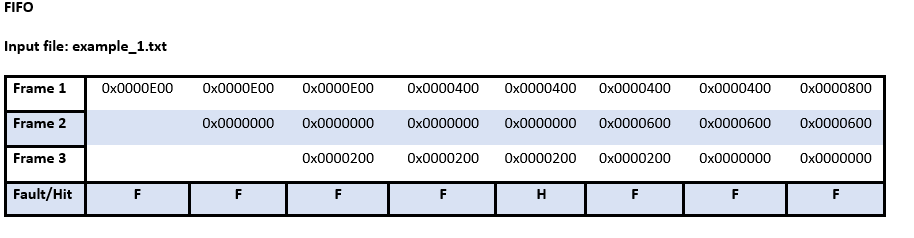
\includegraphics[scale=0.6]{fifo}
\newpage

\subsection*{Least Recently Used (LRU)}
\addcontentsline{toc}{subsection}{Least Recently Used}
The least recently used page (LRU) replacement algorithm, though similar in name to NRU, differs in the fact that LRU keeps track of page usage over a short period of time, while NRU just looks at the usage in the last clock interval. LRU works on the idea that pages that have been most heavily used in the past few instructions are most likely to be used heavily in the next few instructions too. While LRU can provide near-optimal performance in theory (almost as good as Adaptive Replacement Cache), it is rather expensive to implement in practice. There are a few implementation methods for this algorithm that try to reduce the cost yet keep as much of the performance as possible.
\\*
\\*
The most expensive method is the linked list method, which uses a linked list containing all the pages in memory. At the back of this list is the least recently used page, and at the front is the most recently used page. The cost of this implementation lies in the fact that items in the list will have to be moved about every memory reference, which is a very time-consuming process.
Another method that requires hardware support is as follows: suppose the hardware has a 64-bit counter that is incremented at every instruction. Whenever a page is accessed, it acquires the value equal to the counter at the time of page access. Whenever a page needs to be replaced, the operating system selects the page with the lowest counter and swaps it out. With present hardware, this is not feasible because the OS needs to examine the counter for every page in the cache memory. Because of implementation costs, one may consider algorithms (like those that follow) that are similar to LRU, but which offer cheaper implementations.
\\*
\\*
One important advantage of the LRU algorithm is that it is amenable to full statistical analysis. It has been proven, for example, that LRU can never result in more than N-times more page faults than OPT algorithm, where N is proportional to the number of pages in the managed pool.
\\*
\\*
On the other hand, LRU's weakness is that its performance tends to degenerate under many quite common reference patterns. For example, if there are N pages in the LRU pool, an application executing a loop over array of N + 1 pages will cause a page fault on each and every access. As loops over large arrays are common, much effort has been put into modifying LRU to work better in such situations. Many of the proposed LRU modifications try to detect looping reference patterns and to switch into suitable replacement algorithm, like Most Recently Used (MRU).
\\*
LRU is a conservative algorithm, so it is (k/(k-h+1)) competitive.
\\*
\\*
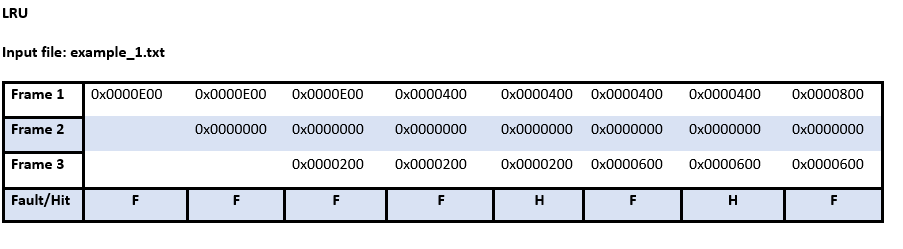
\includegraphics[scale=0.6]{lru}
\newpage

\subsection*{Least Frequently Used (LFU)}
\addcontentsline{toc}{subsection}{Least Frequently Used}
Page with the smallest count is the one which will be selected for replacement. This algorithm suffers from the situation in which a page is used heavily during the initial phase of a process, but then is never used again.
\\*
\\*
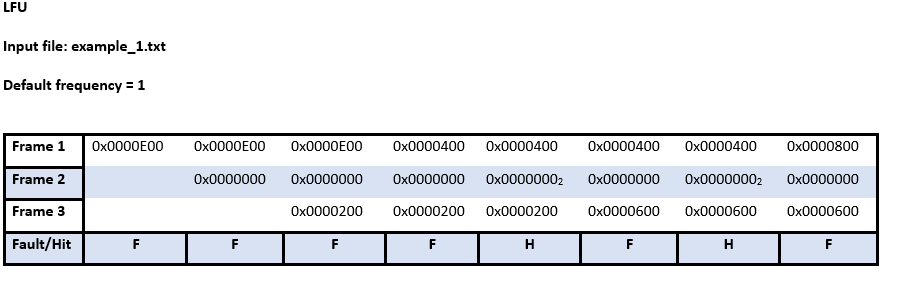
\includegraphics[scale=0.6]{lfu}
\newpage

\subsection*{Most Frequently Used (MFU)}
\addcontentsline{toc}{subsection}{Most Frequently Used}
This algorithm is based on the argument that the page with the smallest count was probably just brought in and has yet to be used[7].
\\*
\\*
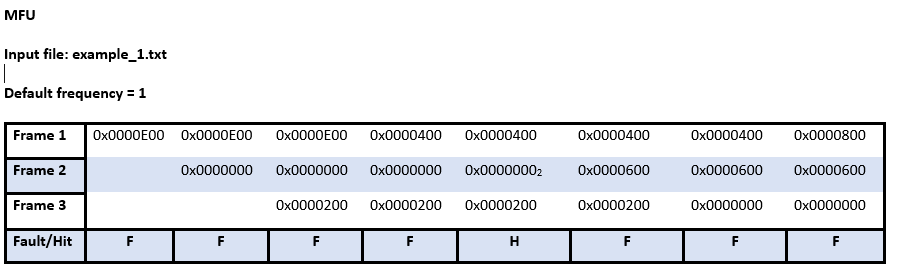
\includegraphics[scale=0.6]{mfu}
\newpage

\subsection*{Clock}
\addcontentsline{toc}{subsection}{Clock}
Clock is a more efficient version of FIFO than Second-chance because pages don't have to be constantly pushed to the back of the list, but it performs the same general function as Second-Chance. The clock algorithm keeps a circular list of pages in memory, with the "hand" (iterator) pointing to the last examined page frame in the list. When a page fault occurs and no empty frames exist, then the R (referenced) bit is inspected at the hand's location. If R is 0, the new page is put in place of the page the "hand" points to, otherwise the R bit is cleared. Then, the clock hand is incremented and the process is repeated until a page is replaced[8].
\\*
Clock is a conservative algorithm, so it is (k/(k-h+1)) competitive.
\\*
\\*
\textbf{Variants of the clock}
\\*
GCLOCK: Generalized clock page replacement algorithm.
\\*
\\*
Clock-Pro keeps a circular list of information about recently referenced pages, including all M pages in memory as well as the most recent M pages that have been paged out. This extra information on paged-out pages, like the similar information maintained by ARC, helps it work better than LRU on large loops and one-time scans.
\\*
\\*
WSclock. The "aging" algorithm and the "WSClock" algorithm are probably the most important page replacement algorithms in practice.
\\*
\\*
Clock with Adaptive Replacement (CAR) is a page replacement algorithm that has performance comparable to ARC, and substantially outperforms both LRU and CLOCK. The algorithm CAR is self-tuning and requires no user-specified magic parameters.
\\*
\\*
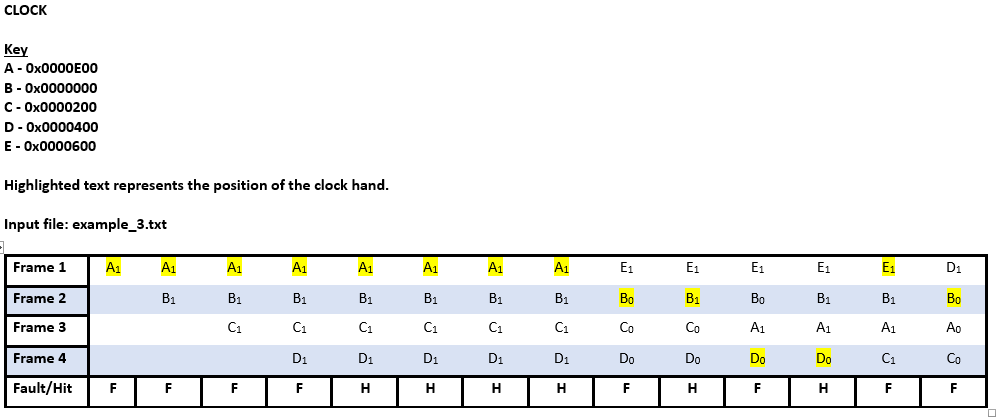
\includegraphics[scale=0.6]{clock}
\newpage

\subsection*{Second Chance}
\addcontentsline{toc}{subsection}{Second Chance}
A modified form of the FIFO page replacement algorithm, known as the Second-chance page replacement algorithm, fares relatively better than FIFO at little cost for the improvement. It works by looking at the front of the queue as FIFO does, but instead of immediately paging out that page, it checks to see if its referenced bit is set. If it is not set, the page is swapped out. Otherwise, the referenced bit is cleared, the page is inserted at the back of the queue (as if it were a new page) and this process is repeated. This can also be thought of as a circular queue. If all the pages have their referenced bit set, on the second encounter of the first page in the list, that page will be swapped out, as it now has its referenced bit cleared. If all the pages have their reference bit set then second chance algorithm degenerates into pure FIFO.
\\*
\\*
As its name suggests, Second-chance gives every page a "second-chance" – an old page that has been referenced is probably in use, and should not be swapped out over a new page that has not been referenced.
\\*
\\*
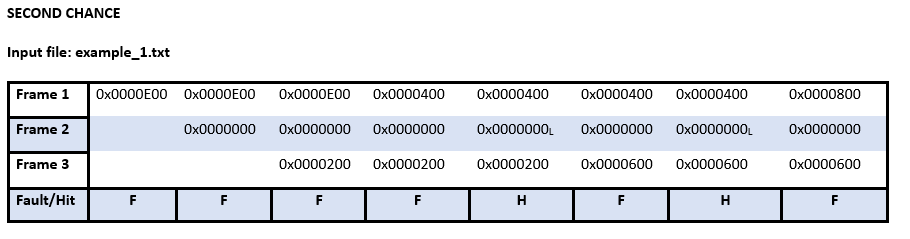
\includegraphics[scale=0.6]{second_chance}
\newpage

\subsection*{Random}
\addcontentsline{toc}{subsection}{Random}
Random replacement algorithm replaces a random page in memory. This eliminates the overhead cost of tracking page references. Usually it fares better than FIFO, and for looping memory references it is better than LRU, although generally LRU performs better in practice. OS/390 uses global LRU approximation and falls back to random replacement when LRU performance degenerates, and the Intel i860 processor used a random replacement policy.
\newpage

\section*{LEARNING OUTCOMES}
\addcontentsline{toc}{section}{LEARNING OUTCOMES}
\begin{enumerate}
\item We learnt about the various topics of memory management. Paging, Demand Paging, Virtual memory, page tables and page replacement to name a few.
\\*
\item Since we were given an incomplete skeleton we learnt about the lifecycle of virtual memory implementation, i.e. what is required and how various components should be linked together to successfully simulate virtual memory implementations. 
\\*
\item We learnt about the pros, cons and the implementation procedure of multiple page replacement algorithms.
\\*
\item Initially, we came up with a new page replacement algorithm which would evict pages from memory based on the frequency associated with a page present in memory. The frequency of that page would be incremented every time there was a hit on that particular page. Recently, we discovered that such an algorithm exists and is known as the “Least Frequently Used” algorithm.
\\*
\item We understood the importance of good documentation and code maintenance. The skeleton code provided had zero documentation and no documentation was provided online. Understanding the given skeleton code was extremely difficult and time consuming.
\\*
\item We learnt how to make a system execute in two modes. Our code is written in such a way that by simply turning off a flag we can switch between execution modes.
\\*
\item We experienced first-hand the difficulties associated with using and modifying code written by a third party.
\end{enumerate}
\newpage

\section*{CONCLUSION}
\addcontentsline{toc}{section}{CONCLUSION}
\subsection*{ALGORITHM COMPARISON}
\addcontentsline{toc}{subsection}{ALGORITHM COMPARISON}
\textbf{Input trace file: trace1000.txt}
\\*
\\*
\textbf{Number of Memory Frames: 64}
\\*
\\*
\textbf{Total number of memory references: 1000}
\\*
\\*
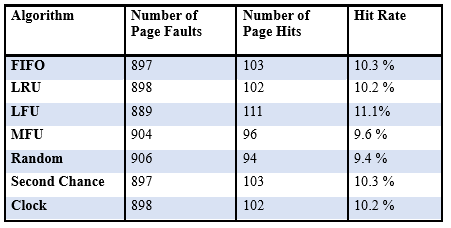
\includegraphics[scale=1.2]{compare}
\\*
\\*
Hit rate is low since the given input file was designed to be the worst case scenario's for every algorithm. For this particular input the least frequently used algorithm has the highest efficiency.

\subsection*{CHALLENGES FACED}
\addcontentsline{toc}{subsection}{CHALLENGES FACED}
\begin{enumerate}
\item \textbf{Understanding the given skeleton code:} The given code had almost no documentation. The biggest challenge was to understand what we had been given. It took us quite a long time to figure out what exactly was happening.
\\*
\item \textbf{Modifying Existing Code:} We were required to make changes in multiple files of the application. Aside from the fault handler, the second most important change was creating the correct structure for page's in the page table and main memory
\\*
\item \textbf{Creating the Fault Handler:} Writing a fault handler implementation which was capable of using multiple algorithms for page replacement
\\*
\item \textbf{Algorithm Implementation:} First, we had to understand each algorithm. Second, we had to figure out that algorithm's implementation in vmsim.
\\*
\item \textbf{Not Recently Used algorithm:} This algorithm requires the knowledge of clock cycle time. Vmsim doesn't provide a complete machine simulation like nachOS. We tried to create a machine folder and make our code run on the simulated clock cycles but we were unsuccessful.

\end{enumerate}

\newpage
 \begin{thebibliography}{1}

  \bibitem{link1} http://www.washington.edu

  \bibitem{link2} http://www.cs.sfu.ca/CourseCentral/300/zonghuag/projects/2011fallproject3.pdf

  \bibitem{link3} http://en.wikipedia.org/wiki/Paging
   
  \bibitem{link5} http://en.wikipedia.org/wiki/Pagereplacementalgorithm
  
  \bibitem{link6} http://en.wikipedia.org/wiki/Memorymanagement
  
  \bibitem{link7} http://en.wikipedia.org/wiki/Virtualmemory
  
  \bibitem{link8} http://www.tutorialspoint.com/operatingsystem/osvirtualmemory.htm
  
  \bibitem{link9} http://www.cs.utexas.edu/users/witchel/372/lectures/16.PageReplacementAlgos.pdf
  
    
  \end{thebibliography}

\end{document}
